%%%%%%%%%%%%%%%%%%%%%%%%%%%%%%%%%%%%%%%%%%%%%%%%%%%%%%%%%%%%%%%%%%%%%%%%%%%%%%%%
% Clasificación de imágenes: anime, caricaturas y personas
%%%%%%%%%%%%%%%%%%%%%%%%%%%%%%%%%%%%%%%%%%%%%%%%%%%%%%%%%%%%%%%%%%%%%%%%%%%%%%%%

\documentclass[letterpaper, 10 pt, conference]{ieeeconf}

\IEEEoverridecommandlockouts
\overrideIEEEmargins

%-------------------------------------------------------------------------------
% Paquetes
%-------------------------------------------------------------------------------

\usepackage[utf8]{inputenc}
\usepackage[T1]{fontenc}
\usepackage[spanish, es-nodecimaldot]{babel}
\usepackage{graphicx}
\usepackage{amsmath}
\usepackage{amssymb}
\usepackage{booktabs}
\usepackage{array}
\usepackage{float}
\usepackage{url}

% Marca visible para las partes que aún no se escriben (buscar "PENDIENTE")
\newcommand{\pendiente}[1]{\textbf{[PENDIENTE: #1]}}

%-------------------------------------------------------------------------------
% Título
%-------------------------------------------------------------------------------

\title{\LARGE \bf
Clasificación de imágenes de anime, caricaturas y personas mediante redes neuronales convolucionales
}

%-------------------------------------------------------------------------------
% Autor
%-------------------------------------------------------------------------------

\author{
Manuel Bajos Rivera, A01711581
}

%-------------------------------------------------------------------------------
% Documento
%-------------------------------------------------------------------------------

\begin{document}

\maketitle
\thispagestyle{empty}
\pagestyle{empty}

%%%%%%%%%%%%%%%%%%%%%%%%%%%%%%%%%%%%%%%%%%%%%%%%%%%%%%%%%%%%%%%%%%%%%%%%%%%%%%%%
% ABSTRACT
%%%%%%%%%%%%%%%%%%%%%%%%%%%%%%%%%%%%%%%%%%%%%%%%%%%%%%%%%%%%%%%%%%%%%%%%%%%%%%%%

\begin{abstract}

En este documento se estudia la clasificación automática de imágenes en tres categorías: anime, caricaturas (cartoon) y personas (human). Para ello se utiliza el conjunto de datos Anime vs Cartoon vs Human obtenido de Kaggle, compuesto por 8,917 imágenes distribuidas de forma casi balanceada entre las tres clases.

El estudio se enfoca en un problema de clasificación multiclase de imágenes. Se implementa primero una red neuronal convolucional propia con TensorFlow y Keras como modelo base, y posteriormente se mejora mediante técnicas de regularización, ajuste de hiperparámetros y transferencia de aprendizaje con una arquitectura preentrenada. Un análisis exploratorio previo identificó 383 imágenes duplicadas exactas y diferencias marcadas de resolución y peso entre clases, que podrían permitir al modelo clasificar por atajos y no por contenido.

\pendiente{resumir los resultados finales: exactitud en prueba de la CNN base, de la CNN mejorada y del modelo con transferencia de aprendizaje, y qué cambios funcionaron.}

\end{abstract}

%%%%%%%%%%%%%%%%%%%%%%%%%%%%%%%%%%%%%%%%%%%%%%%%%%%%%%%%%%%%%%%%%%%%%%%%%%%%%%%%
% PROBLEMÁTICA
%%%%%%%%%%%%%%%%%%%%%%%%%%%%%%%%%%%%%%%%%%%%%%%%%%%%%%%%%%%%%%%%%%%%%%%%%%%%%%%%

\section{Problemática}

Distinguir automáticamente el estilo visual de una imagen (dibujo de anime, caricatura occidental o fotografía de una persona) es un problema de clasificación de imágenes que puede resultar útil, por ejemplo, para organizar colecciones de imágenes o filtrar contenido. Las tres categorías comparten elementos como rostros, colores y contornos, pero difieren en el trazo, la textura y la composición, por lo que no es una tarea trivial para un clasificador basado en reglas.

Dado esto, se plantea un problema de clasificación multiclase cuya meta es predecir, a partir de una imagen a color, a cuál de las tres clases pertenece: \texttt{anime}, \texttt{cartoon} o \texttt{human}. Las variables de entrada son los píxeles de la imagen y la variable objetivo es la etiqueta de la clase.

Dado que los datos son imágenes, se emplean redes neuronales convolucionales (CNN), que son capaces de aprender de forma automática jerarquías de características visuales a partir de los píxeles.

%%%%%%%%%%%%%%%%%%%%%%%%%%%%%%%%%%%%%%%%%%%%%%%%%%%%%%%%%%%%%%%%%%%%%%%%%%%%%%%%
% DATOS
%%%%%%%%%%%%%%%%%%%%%%%%%%%%%%%%%%%%%%%%%%%%%%%%%%%%%%%%%%%%%%%%%%%%%%%%%%%%%%%%

\section{Datos}

El conjunto de datos utilizado corresponde a Anime vs Cartoon vs Human, disponible en Kaggle \cite{dataset}. Contiene 8,917 imágenes organizadas en tres carpetas, una por clase. Es un conjunto de datos reales y no un ejemplo de clase. La Tabla~\ref{tab:clases} resume su composición.

\begin{table}[H]
\caption{Composición del conjunto de datos original}
\label{tab:clases}
\centering
\footnotesize
\begin{tabular}{lcccc}
\hline
\textbf{Clase} & \textbf{Imágenes} & \textbf{Formato} & \textbf{Ancho típico} & \textbf{Peso típico} \\
\hline
\texttt{anime}   & 3,004 & JPEG & 68 px   & 4 KB \\
\texttt{cartoon} & 2,913 & PNG y JPEG & 258 px  & 55 KB \\
\texttt{human}   & 3,000 & PNG  & 1,024 px & 1,334 KB \\
\hline
\end{tabular}
\end{table}

La Figura~\ref{fig:conteo} muestra que las clases están casi balanceadas, con entre 2,913 y 3,004 imágenes por clase, por lo que la exactitud (accuracy) es una métrica adecuada para evaluar el modelo.

\begin{figure}[H]
    \centering
    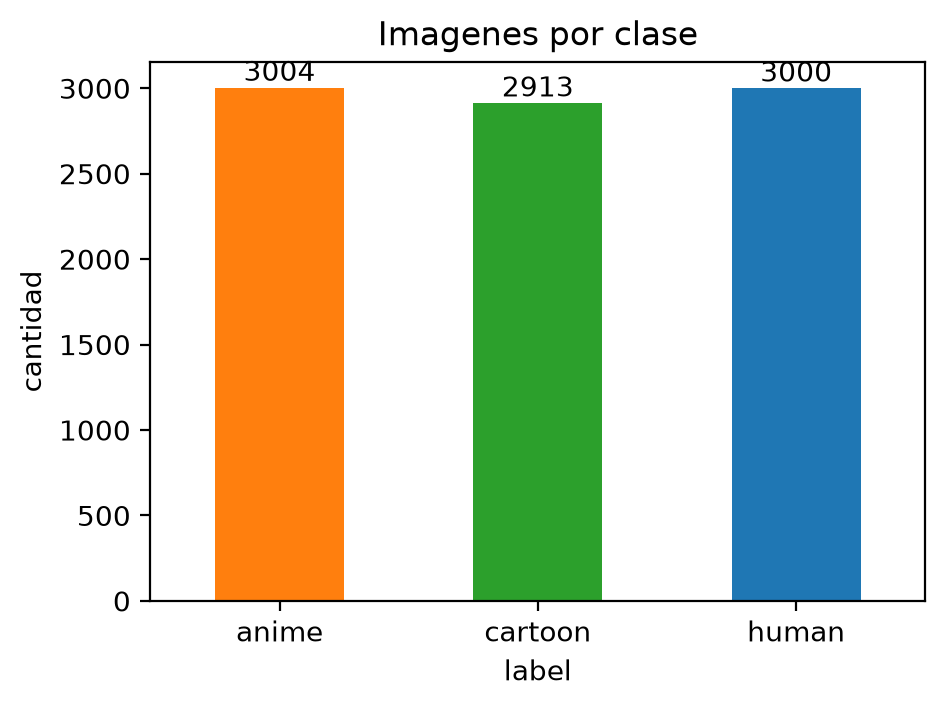
\includegraphics[width=0.7\columnwidth]{figuras/conteo_clases.png}
    \caption{Número de imágenes por clase en el conjunto original.}
    \label{fig:conteo}
\end{figure}

Las imágenes tienen características muy distintas entre clases. Las imágenes de anime son miniaturas cuadradas de entre 25 y 189 píxeles de ancho. Las de cartoon van de 74 a 519 píxeles de ancho y su relación de aspecto varía entre 0.37 y 5.35, de modo que solamente el 12\% son cuadradas. Las de human son siempre cuadradas de 1,024 $\times$ 1,024 píxeles.

Además, las imágenes de cartoon mezclan tres modos de color: 653 en RGB, 2,186 en RGBA y 74 con paleta indexada. Ninguna de las imágenes con canal alfa presenta transparencia real, por lo que su conversión a RGB no altera el contenido.

%%%%%%%%%%%%%%%%%%%%%%%%%%%%%%%%%%%%%%%%%%%%%%%%%%%%%%%%%%%%%%%%%%%%%%%%%%%%%%%%
% ANALISIS EXPLORATORIO
%%%%%%%%%%%%%%%%%%%%%%%%%%%%%%%%%%%%%%%%%%%%%%%%%%%%%%%%%%%%%%%%%%%%%%%%%%%%%%%%

\section{Análisis exploratorio}

Antes del entrenamiento se realizó un análisis de la integridad, la resolución, el color y el contenido de las imágenes. Se verificó que ninguna de las 8,917 imágenes estuviera corrupta.

La Figura~\ref{fig:muestras} presenta una muestra aleatoria de imágenes de cada clase, con su resolución original. Se observa que tanto anime como human son retratos de rostros recortados, mientras que cartoon incluye personajes de cuerpo completo, escenas y capturas de pantalla con márgenes. Esto indica que, además del estilo, la composición de la imagen también diferencia a las clases.

\begin{figure}[H]
    \centering
    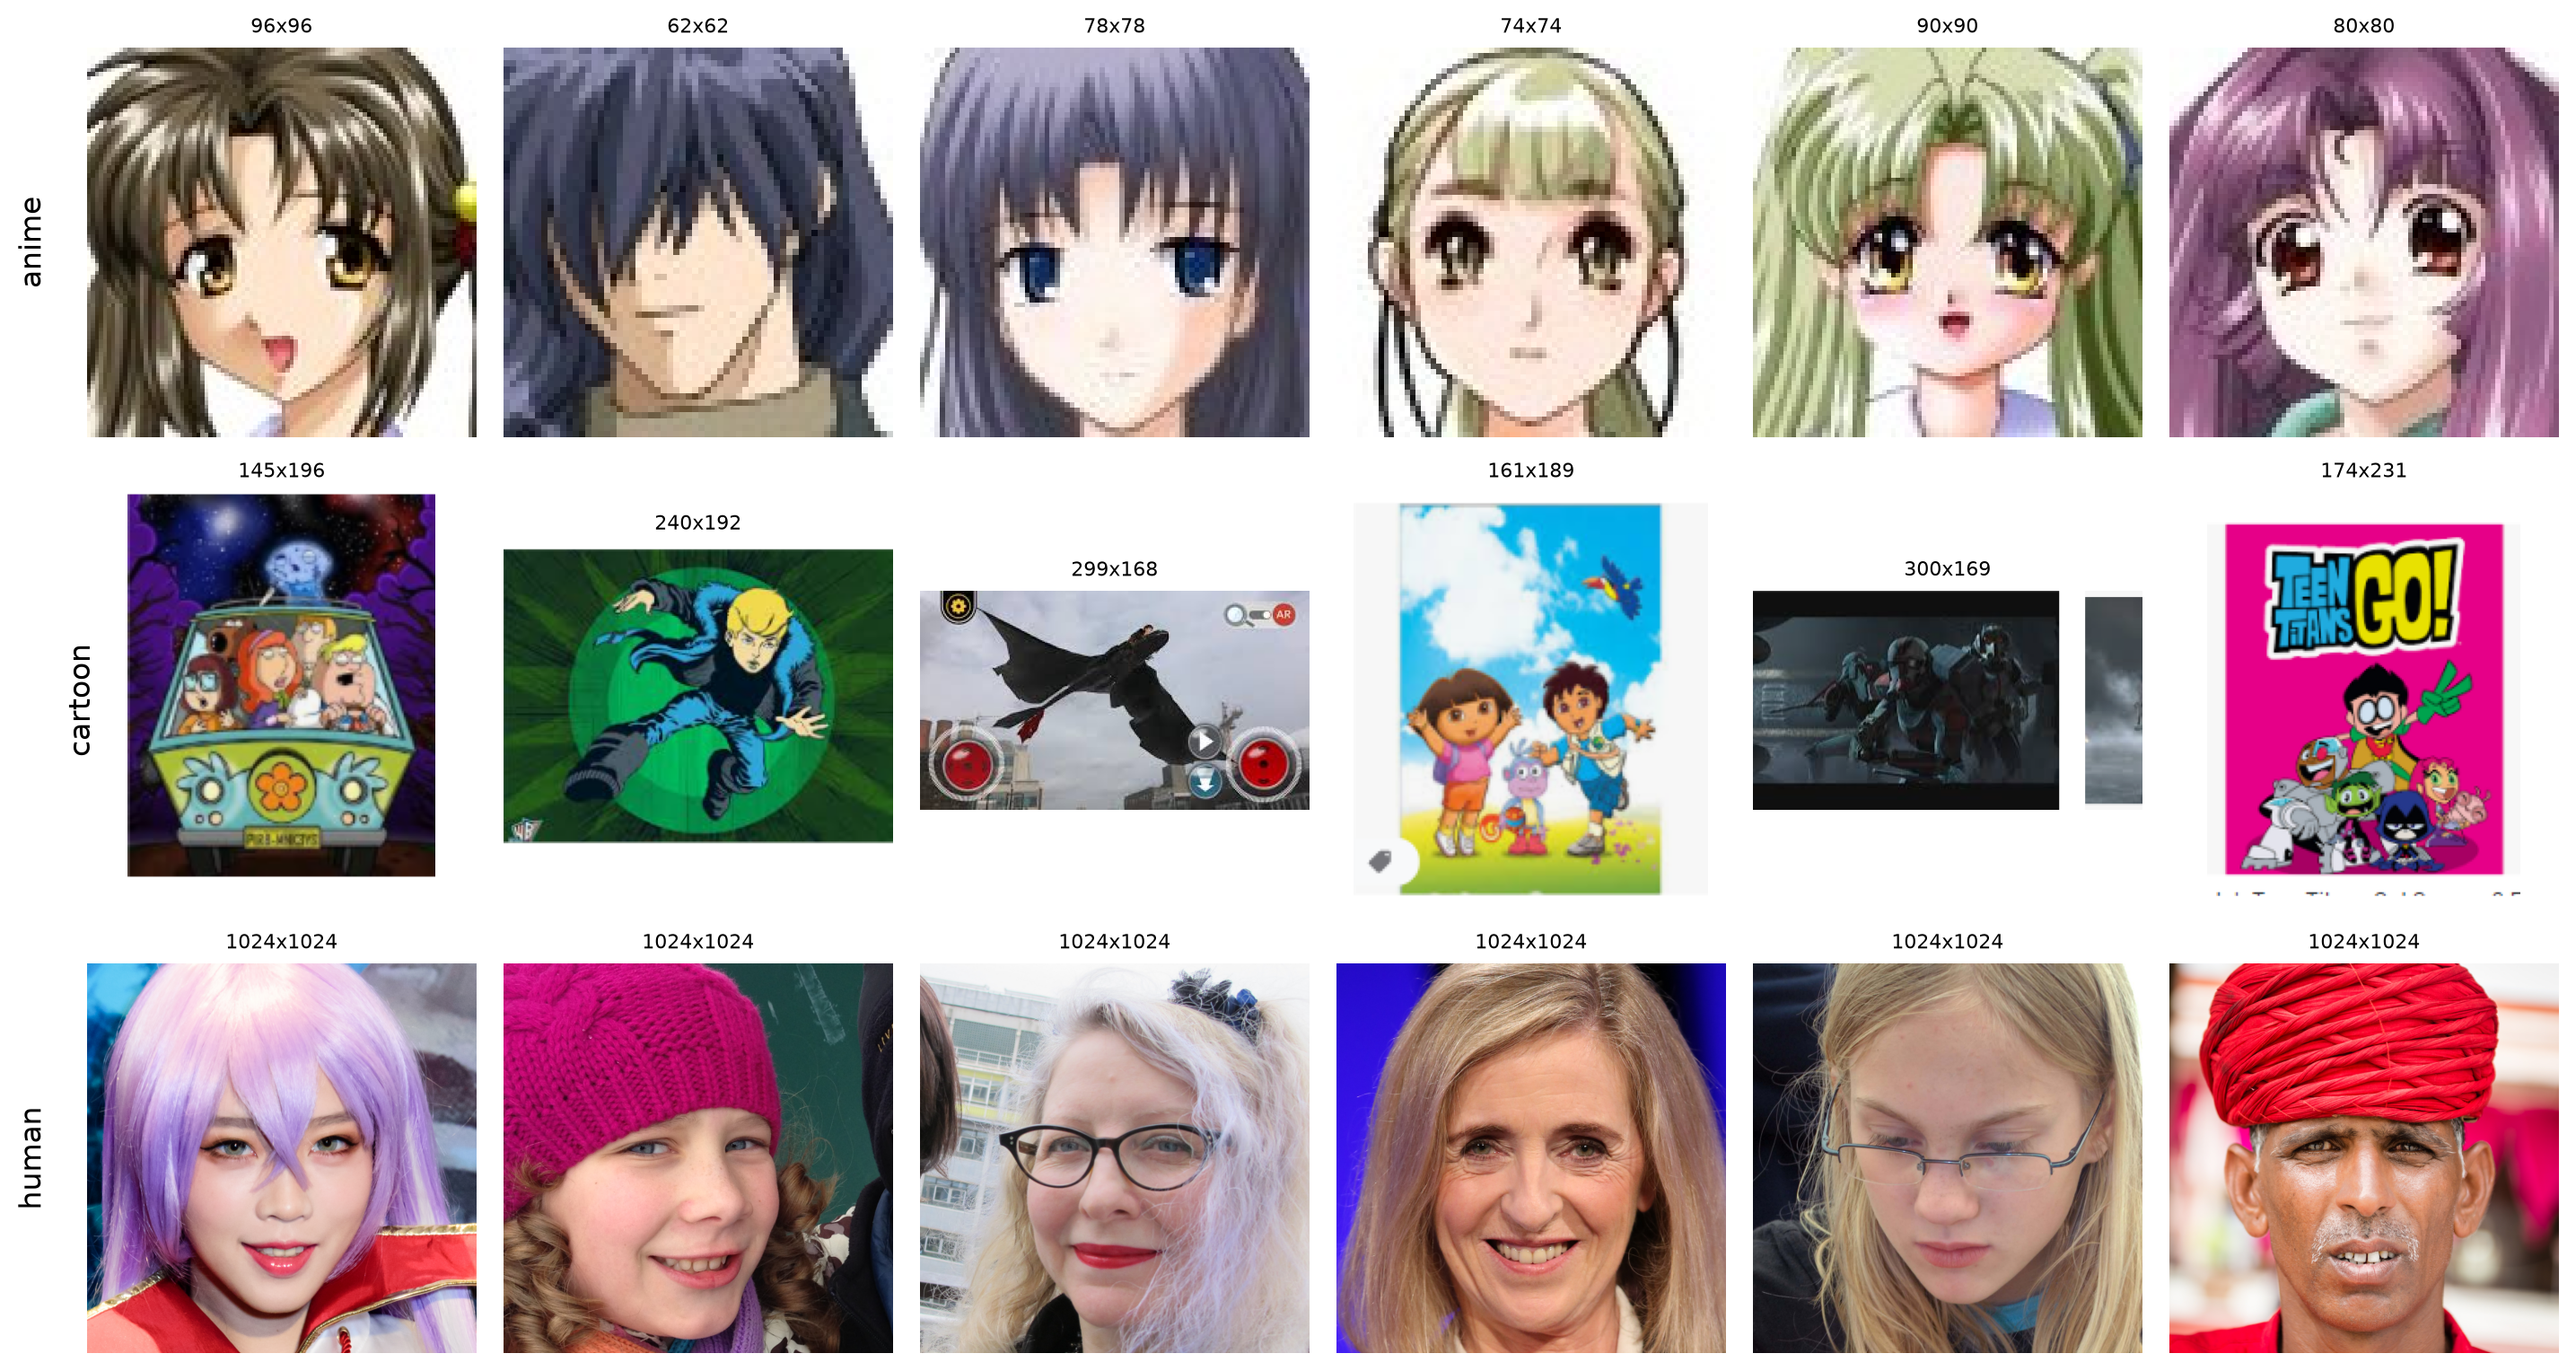
\includegraphics[width=\columnwidth]{figuras/muestras.png}
    \caption{Muestra aleatoria de imágenes por clase. El título de cada imagen indica su resolución original.}
    \label{fig:muestras}
\end{figure}

\subsection{Riesgo de atajos por resolución y peso}

La Figura~\ref{fig:tamano} compara el valor típico (mediana) de cada clase. Las imágenes de human son aproximadamente 15 veces más anchas y 300 veces más pesadas que las de anime. Esta diferencia es tan marcada que, por sí sola, permitiría identificar la clase sin observar el contenido de la imagen.

\begin{figure}[H]
    \centering
    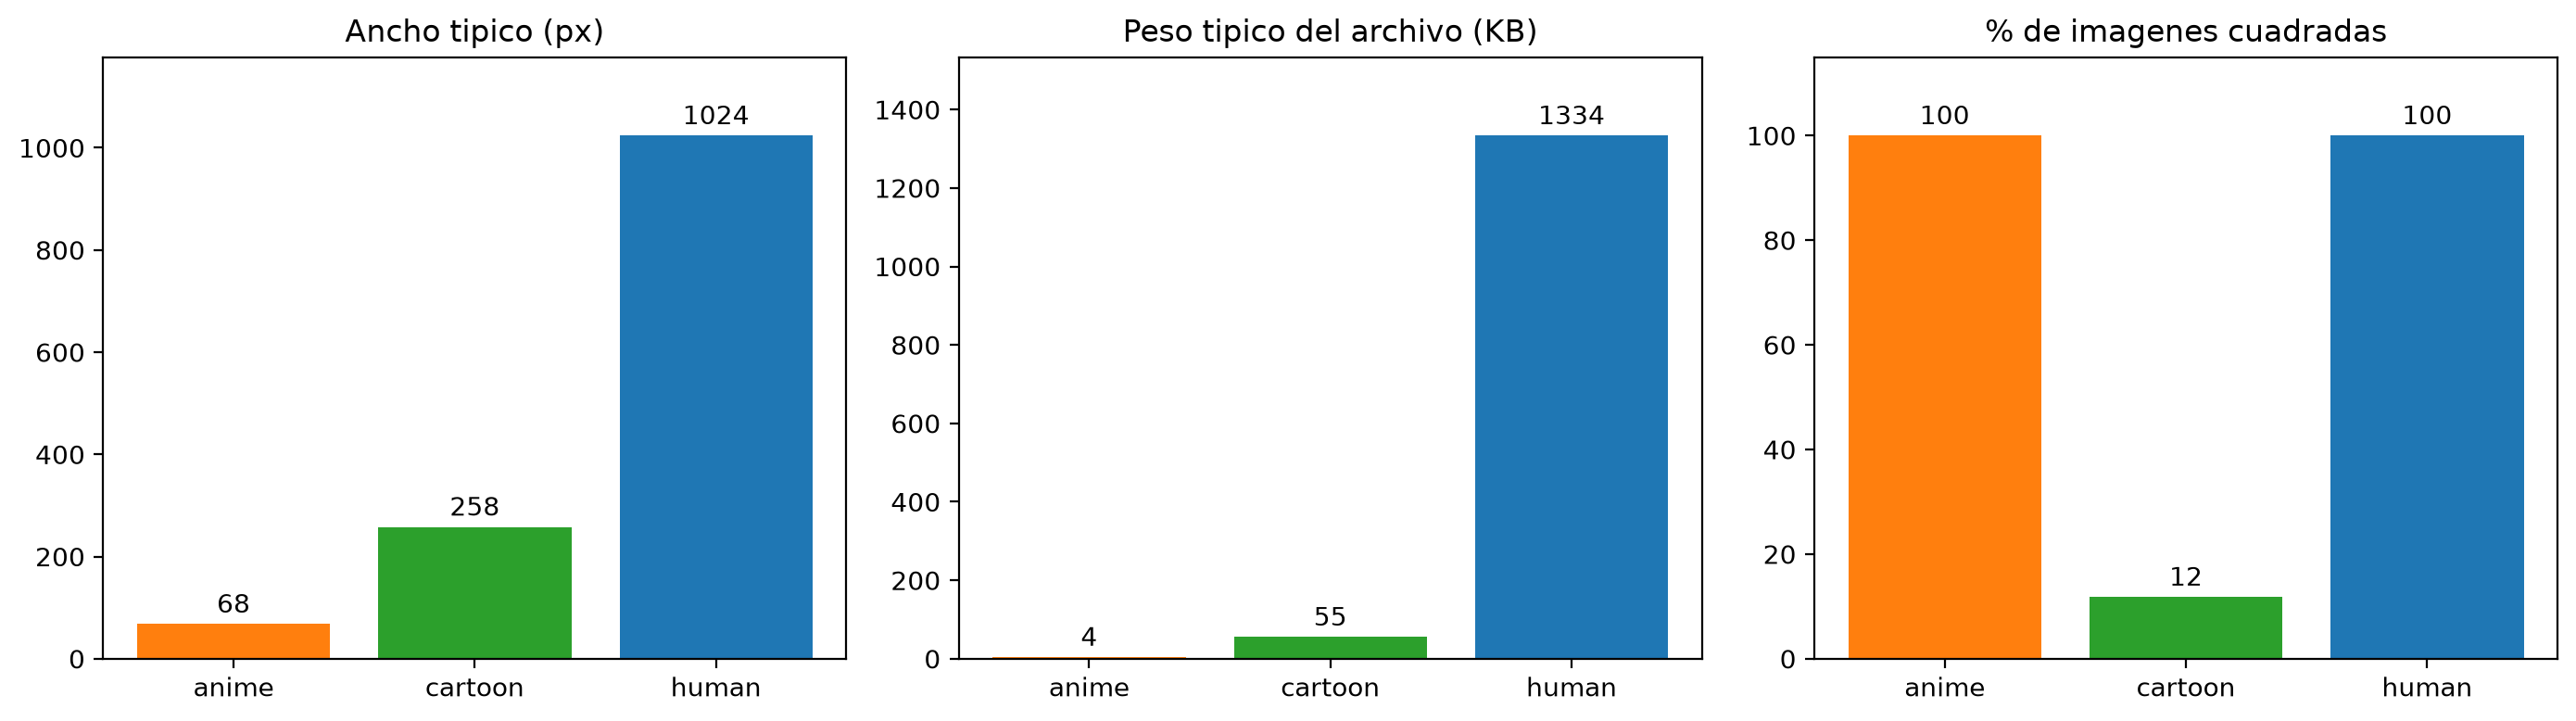
\includegraphics[width=\columnwidth]{figuras/tamano_por_clase.png}
    \caption{Ancho típico, peso típico del archivo y porcentaje de imágenes cuadradas por clase.}
    \label{fig:tamano}
\end{figure}

Esto representa un riesgo, ya que un modelo podría aprender un atajo basado en la nitidez o la resolución y no en las características visuales de cada categoría, lo que produciría una exactitud alta pero engañosa. Para mitigarlo, todas las imágenes se redimensionan a un mismo tamaño antes de entrenar, y se evalúa el modelo con imágenes externas que no provienen del conjunto de datos.

Una diferencia similar aparece en el color. La Figura~\ref{fig:color} muestra que las imágenes de human son en promedio más oscuras (medias de los canales R, G y B de 0.52, 0.42 y 0.38) que las de anime (0.64, 0.54 y 0.51) y cartoon (0.61, 0.58 y 0.55), lo que constituye otra señal que el modelo podría aprovechar.

\begin{figure}[H]
    \centering
    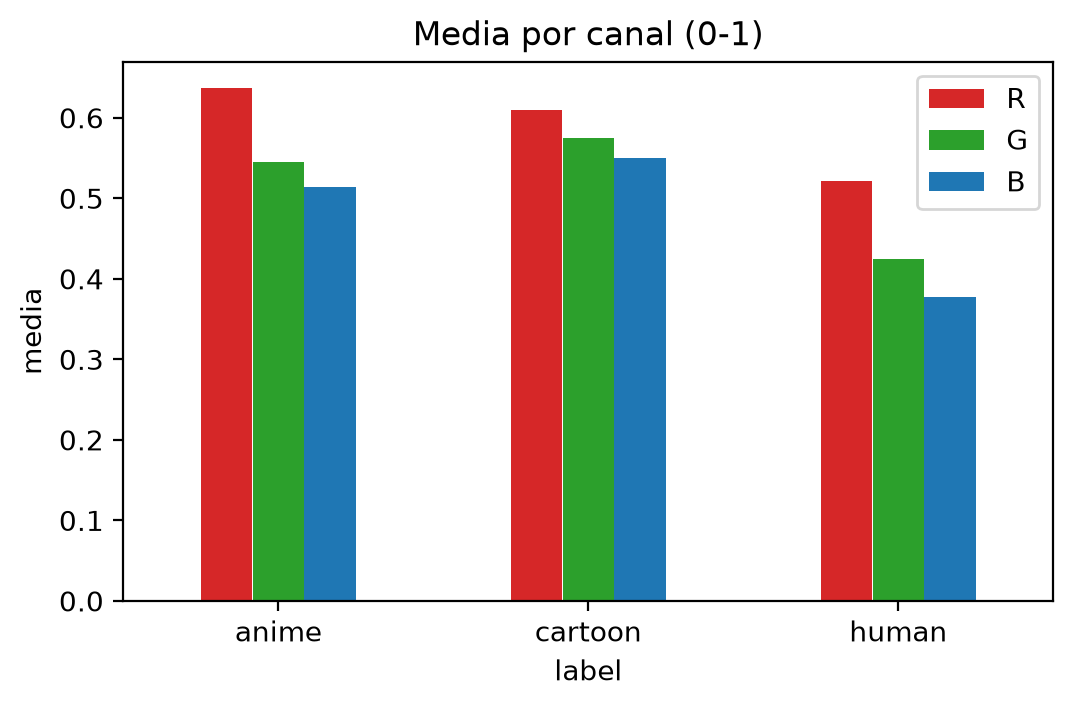
\includegraphics[width=0.7\columnwidth]{figuras/color_medio.png}
    \caption{Media de cada canal de color por clase, sobre una muestra de 300 imágenes por clase.}
    \label{fig:color}
\end{figure}

\subsection{Imágenes duplicadas}

Se calculó el resumen criptográfico MD5 del contenido de cada archivo para detectar duplicados exactos. Se encontraron 712 imágenes involucradas en 329 grupos de duplicados, es decir, 383 imágenes sobrantes. Todas pertenecen a la clase anime y ningún grupo mezcla clases distintas. La Figura~\ref{fig:dup} muestra algunos ejemplos: son la misma imagen guardada con nombres de archivo diferentes. La mayoría de los grupos son pares, aunque algunos contienen hasta cinco copias.

\begin{figure}[H]
    \centering
    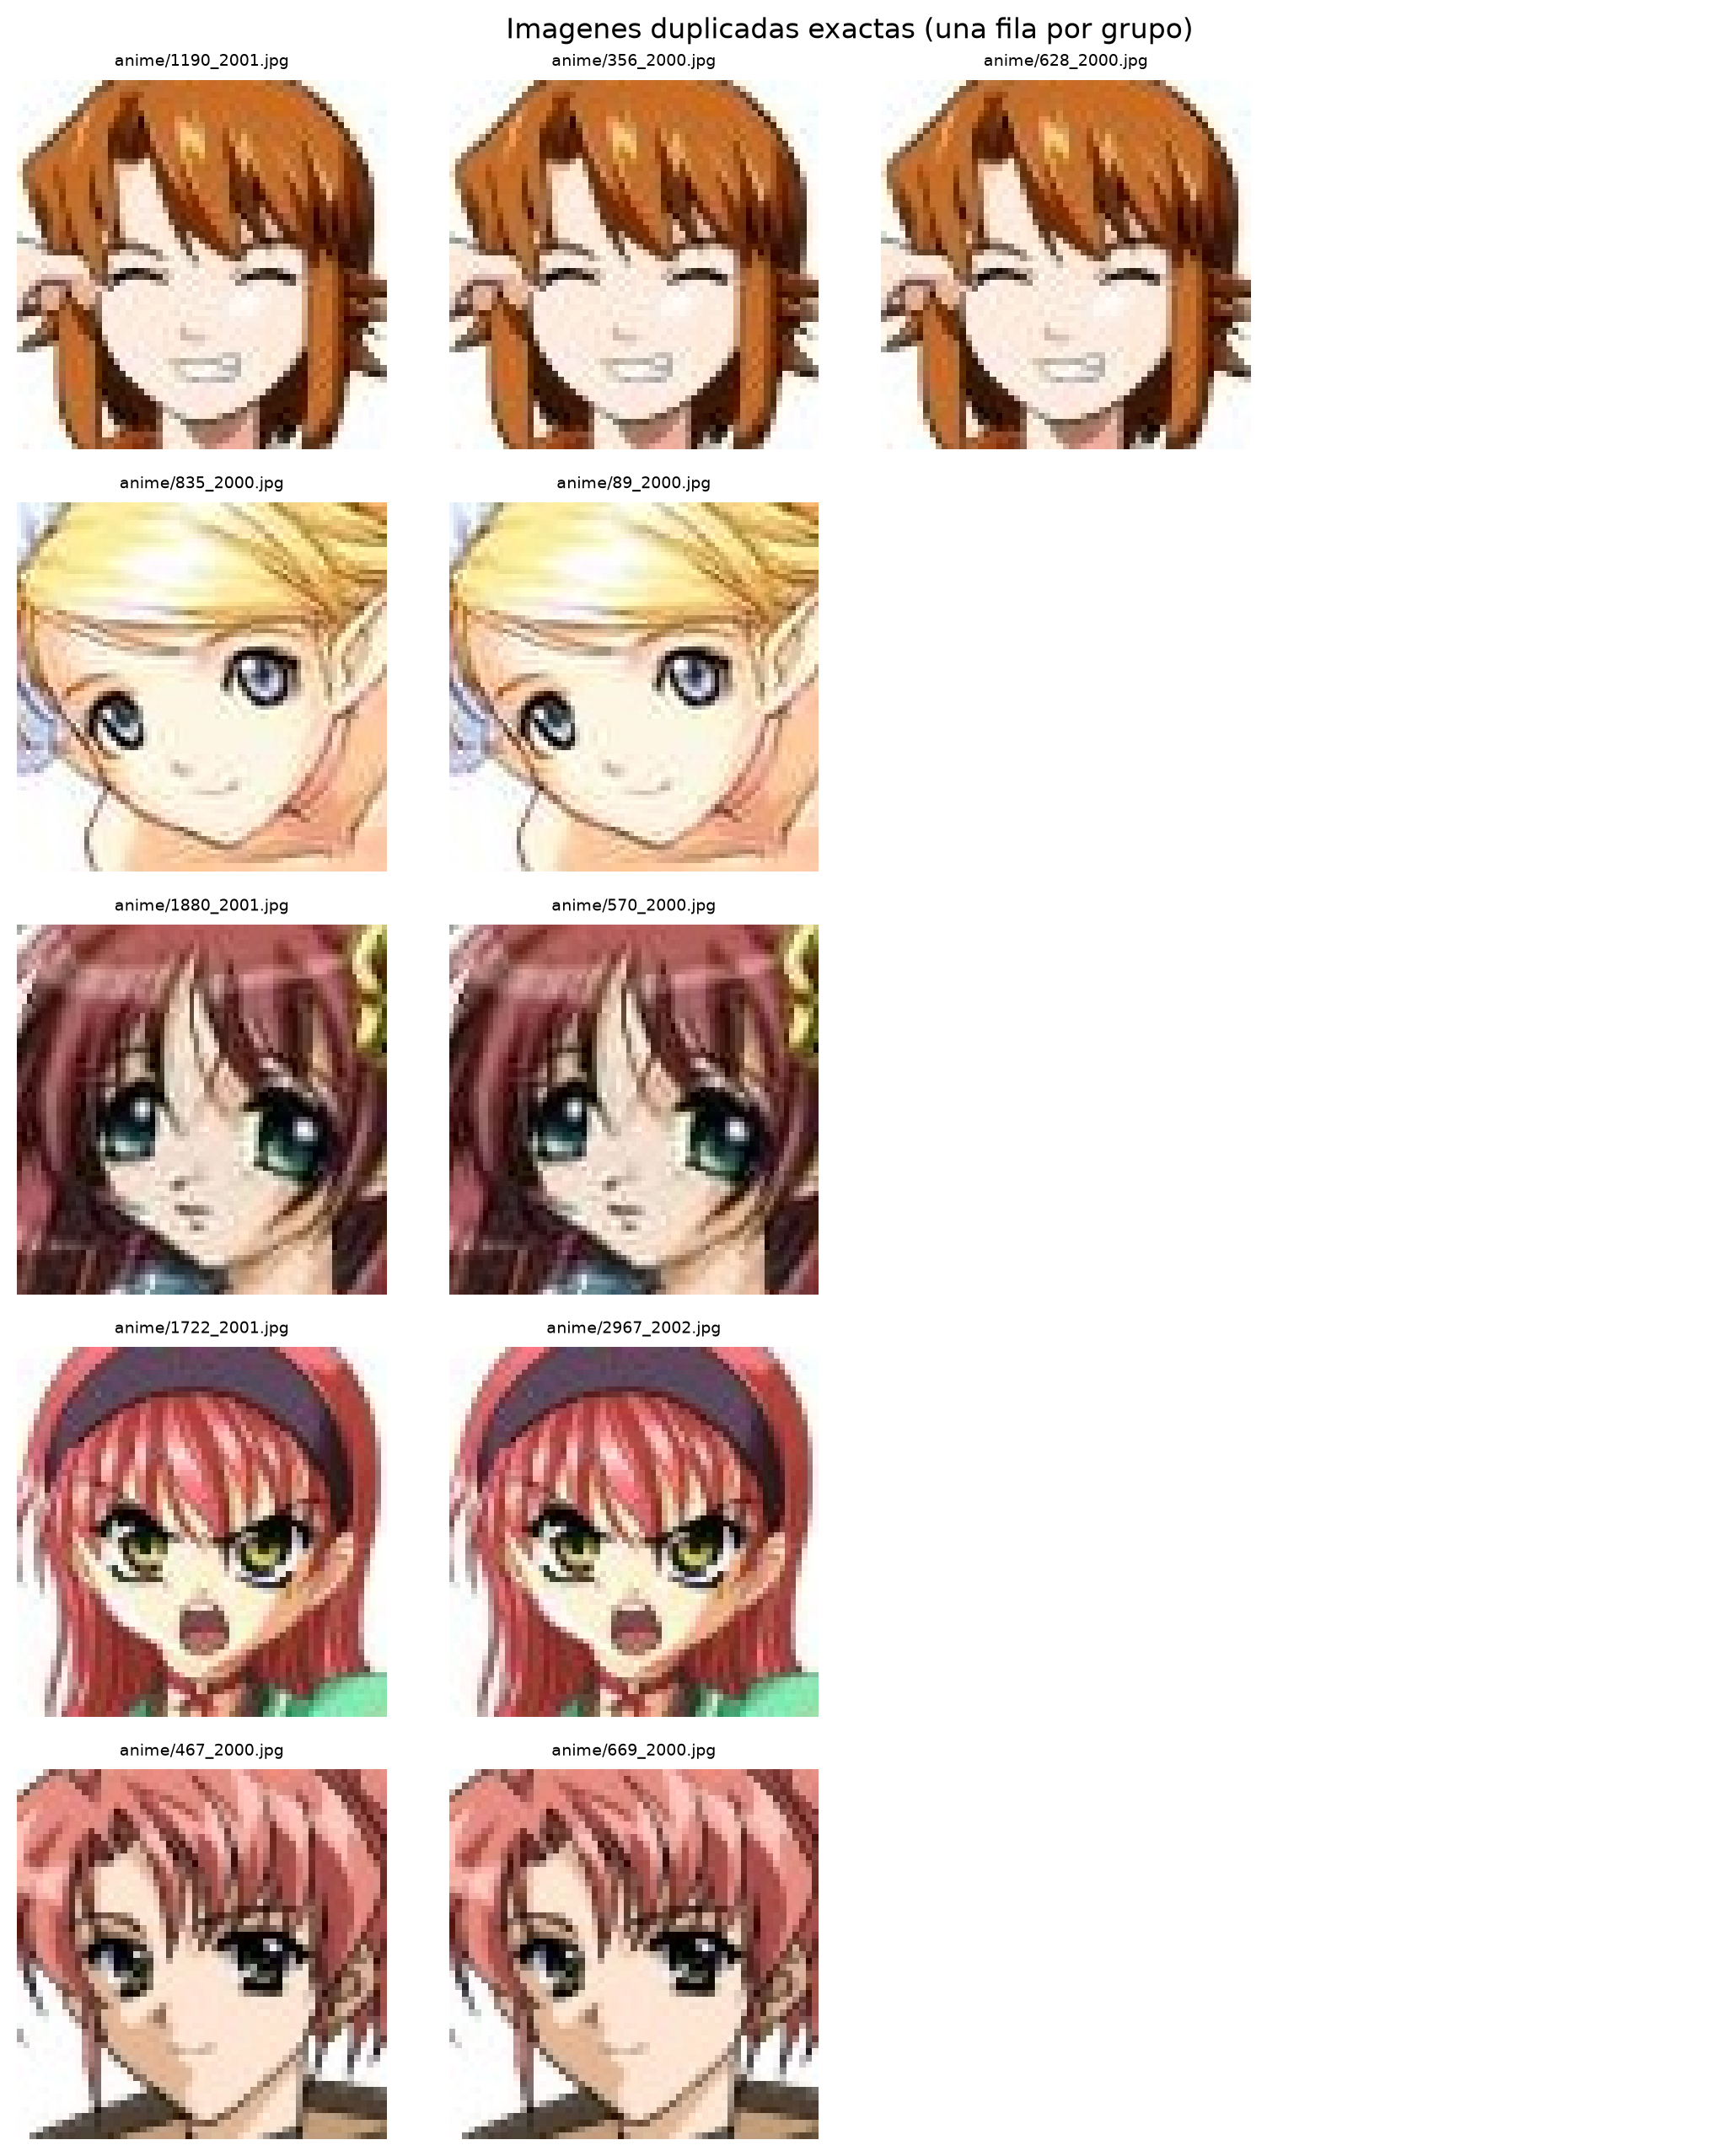
\includegraphics[width=0.85\columnwidth]{figuras/duplicados.png}
    \caption{Ejemplos de grupos de imágenes duplicadas exactas (una fila por grupo).}
    \label{fig:dup}
\end{figure}

Los duplicados deben eliminarse antes de dividir los datos. De lo contrario, una copia podría quedar en el conjunto de entrenamiento y otra en el de prueba, y el modelo habría visto la respuesta durante el entrenamiento, con lo que el desempeño en prueba sería artificialmente alto. Tras la deduplicación el conjunto contiene 2,621 imágenes de anime, 2,913 de cartoon y 3,000 de human (8,534 en total), con un desbalance leve.

%%%%%%%%%%%%%%%%%%%%%%%%%%%%%%%%%%%%%%%%%%%%%%%%%%%%%%%%%%%%%%%%%%%%%%%%%%%%%%%%
% ETL
%%%%%%%%%%%%%%%%%%%%%%%%%%%%%%%%%%%%%%%%%%%%%%%%%%%%%%%%%%%%%%%%%%%%%%%%%%%%%%%%

\section{ETL}

El proceso de extracción, transformación y carga se realizó antes del entrenamiento con el objetivo de obtener un conjunto de datos adecuado para la clasificación. El proyecto se implementó en Python con TensorFlow 2.20 y Keras 3 \cite{tensorflow, keras}, versiones que cuentan con soporte en macOS, Linux y Windows.

La extracción se hizo mediante la biblioteca \texttt{kagglehub}, que descarga el conjunto de datos y lo guarda en una caché local. Posteriormente se construyó una tabla con la ruta y la clase de cada imagen, y se eliminaron los duplicados exactos como se describió en la sección anterior.

\subsection{Partición de los datos}

Sobre las imágenes sin duplicados se realizó una partición estratificada por clase en tres subconjuntos: 70\% para entrenamiento, 15\% para validación y 15\% para prueba, con una semilla fija (42) para que los resultados sean reproducibles. La estratificación mantiene en cada subconjunto la misma proporción de clases que en el total, lo que conserva el leve desbalance de anime. La Tabla~\ref{tab:particion} muestra el resultado.

\begin{table}[H]
\caption{Número de imágenes por clase y partición}
\label{tab:particion}
\centering
\footnotesize
\begin{tabular}{lcccc}
\hline
\textbf{Clase} & \textbf{Entrenamiento} & \textbf{Validación} & \textbf{Prueba} & \textbf{Total} \\
\hline
\texttt{anime}   & 1,834 & 393   & 394   & 2,621 \\
\texttt{cartoon} & 2,039 & 437   & 437   & 2,913 \\
\texttt{human}   & 2,100 & 450   & 450   & 3,000 \\
\hline
\textbf{Total}   & 5,973 & 1,280 & 1,281 & 8,534 \\
\hline
\end{tabular}
\end{table}

La partición se hizo sobre las rutas de las imágenes y antes de transformarlas, de modo que ninguna información de validación o prueba interviene en el entrenamiento. Además, se verificó mediante el resumen MD5 que ninguna imagen aparece en más de una partición. El conjunto de entrenamiento se utiliza para ajustar los parámetros de los modelos, el de validación para monitorear el desempeño y ajustar hiperparámetros, y el de prueba se mantiene aislado y se usa únicamente para reportar el desempeño final.

\subsection{Transformación de las imágenes}

Cada imagen se convierte a RGB de tres canales y se deja en un tamaño único de $128 \times 128$ píxeles, ya que la red convolucional requiere entradas de dimensiones fijas. La reducción se realiza con el método de remuestreo de Lanczos, aplicado de la misma manera a todas las clases, para evitar que la nitidez de la imagen reducida difiera artificialmente entre ellas.

Como las imágenes de cartoon no son cuadradas en su mayoría, se probaron dos estrategias para llegar a un cuadrado:

\begin{itemize}
    \item \textbf{Relleno (padding):} se reduce la imagen conservando su proporción, de modo que su lado mayor mida 128 píxeles, y se centra sobre un lienzo cuadrado rellenado con el color mediano de su propio borde, para que las bandas resultantes sean poco llamativas.
    \item \textbf{Estiramiento (stretch):} se redimensiona directamente a $128 \times 128$, lo que deforma las imágenes no cuadradas.
\end{itemize}

Se comenzó con el relleno. Sin embargo, como solo el 12\% de las imágenes de cartoon son cuadradas y el 100\% de anime y human lo son, el relleno hace que casi todas las imágenes de cartoon tengan bandas y ninguna de las otras clases, lo cual puede convertirse en un atajo para el modelo. Por ello, posteriormente se compara con el estiramiento, que no introduce bordes pero deforma las proporciones. \pendiente{reportar la comparación de resultados entre ambas estrategias.}

\subsection{Carga y almacenamiento en caché}

Las imágenes transformadas se guardan como arreglos de enteros sin signo de 8 bits (\texttt{uint8}) en una caché local, uno por partición y por estrategia de redimensionado. De esta forma, el costo de decodificar y reducir las imágenes originales, en particular las de 1,024 $\times$ 1,024 píxeles de human, se paga una sola vez. El conjunto de entrenamiento ocupa aproximadamente 294 MB en memoria, por lo que cabe completo en la RAM. El procesamiento de las 8,534 imágenes se paraleliza con hilos y tomó 11 segundos en la computadora utilizada. Las etiquetas se codifican como enteros (0 para anime, 1 para cartoon y 2 para human).

La normalización de los píxeles al rango $[0,1]$ se realiza dividiendo entre 255 mediante una capa \texttt{Rescaling} dentro de la CNN propia. Para la arquitectura preentrenada se utiliza el preprocesamiento que ella misma incluye. \pendiente{confirmar al implementar el modelo con transferencia de aprendizaje.}

%%%%%%%%%%%%%%%%%%%%%%%%%%%%%%%%%%%%%%%%%%%%%%%%%%%%%%%%%%%%%%%%%%%%%%%%%%%%%%%%
% MODELOS
%%%%%%%%%%%%%%%%%%%%%%%%%%%%%%%%%%%%%%%%%%%%%%%%%%%%%%%%%%%%%%%%%%%%%%%%%%%%%%%%

\section{Modelos}

\subsection{CNN propia (modelo base)}

\pendiente{describir la arquitectura (bloques convolucionales, pooling, capas densas), la función de pérdida, el optimizador y los hiperparámetros iniciales. Incluir el fundamento de la operación de convolución y de la capa softmax.}

\subsection{Evaluación del modelo base}

\pendiente{curvas de entrenamiento y validación, exactitud en validación y prueba, matriz de confusión y análisis de errores.}

\subsection{Mejoras al modelo}

\pendiente{documentar una a una las mejoras probadas (aumento de datos, Dropout, BatchNorm, regularización L2, early stopping, ajuste de la tasa de aprendizaje y de la arquitectura), cuáles funcionaron y por qué.}

\subsection{Transferencia de aprendizaje}

\pendiente{describir la arquitectura preentrenada utilizada, la cabeza de clasificación añadida, el entrenamiento con la base congelada y el ajuste fino posterior.}

%%%%%%%%%%%%%%%%%%%%%%%%%%%%%%%%%%%%%%%%%%%%%%%%%%%%%%%%%%%%%%%%%%%%%%%%%%%%%%%%
% PREDICCIONES
%%%%%%%%%%%%%%%%%%%%%%%%%%%%%%%%%%%%%%%%%%%%%%%%%%%%%%%%%%%%%%%%%%%%%%%%%%%%%%%%

\section{Predicciones con imágenes nuevas}

\pendiente{probar el modelo con imágenes externas al conjunto de datos y mostrar algunas predicciones, para comprobar que el modelo no depende de la resolución ni del peso del archivo.}

%%%%%%%%%%%%%%%%%%%%%%%%%%%%%%%%%%%%%%%%%%%%%%%%%%%%%%%%%%%%%%%%%%%%%%%%%%%%%%%%
% RESULTADOS
%%%%%%%%%%%%%%%%%%%%%%%%%%%%%%%%%%%%%%%%%%%%%%%%%%%%%%%%%%%%%%%%%%%%%%%%%%%%%%%%

\section{Resultados}

\pendiente{tabla comparativa de exactitud en entrenamiento, validación y prueba para cada modelo, y conclusiones.}

%%%%%%%%%%%%%%%%%%%%%%%%%%%%%%%%%%%%%%%%%%%%%%%%%%%%%%%%%%%%%%%%%%%%%%%%%%%%%%%%
% REFERENCIAS
%%%%%%%%%%%%%%%%%%%%%%%%%%%%%%%%%%%%%%%%%%%%%%%%%%%%%%%%%%%%%%%%%%%%%%%%%%%%%%%%

\begin{thebibliography}{99}

\bibitem{dataset}
hadiepratamatulili, ``Anime vs Cartoon vs Human,'' Kaggle.
[Online]. Available:
\url{https://www.kaggle.com/datasets/hadiepratamatulili/anime-vs-cartoon-vs-human}
[Accessed: Oct. 26, 2026].

\bibitem{tensorflow}
M. Abadi et al., ``TensorFlow: Large-scale machine learning on heterogeneous systems,'' 2015.
[Online]. Available: \url{https://www.tensorflow.org/}

\bibitem{keras}
F. Chollet et al., ``Keras,'' 2015.
[Online]. Available: \url{https://keras.io}

\end{thebibliography}

\end{document}
